\documentclass[a4paper]{article}
\usepackage{fullpage}
\usepackage{amsmath}
\usepackage{amssymb}
\usepackage{bussproofs}
\usepackage{forest}

\usepackage{graphicx}
\graphicspath{ {./images/} }

\newtheorem{lemma}{Lemma}
\newtheorem{theorem}{Theorem}
\setcounter{theorem}{117}
\newtheorem{definition}{Definition}
\newtheorem{proof}{Proof}
\newtheorem{claim}{Claim}
\setcounter{claim}{119}

\newcommand{\MODEL}{\mathcal{M}}
\newcommand{\SUBMODEL}{\mathcal{N}}
\newcommand{\LANGUAGE}{\mathcal{L}}
\newcommand{\TUPLE}[1]{\langle {#1} \rangle}
\newcommand{\SET}[1]{\{ {#1} \}}
\newcommand{\PV}{\varphi}
\newcommand{\QV}{\psi}

\title{PHIL3110 - Exam}
\author{Maxwell Bo}

\begin{document} 

\maketitle

\section*{Part A}

\subsection*{Problem 1}

\begin{enumerate}

    \item

Let $\beta = \SET{ \varphi \mid \varphi \in \Gamma \wedge \varphi \in \Delta }$.

Say there's some $\varphi$ such that $\beta \models \varphi$ but $\varphi \not\in \beta$. If $\varphi \not\in \beta$, then $\varphi \not\in \Gamma$ and $\varphi \not\in \Delta$.\\

    \textsc{Abortive} I looked for a counter-example $\varphi$ that could both be true in two seperate sets, but when stripped of its environment (all the $\psi$s in which $\psi \in \Gamma$ but $\psi \not\in \Delta$, and vice-versa) allowed a derivation to something that was not in $\Gamma$ and $\Delta$. I found this very difficult.\\

    \textsc{Abortive} We'll try reductio ad absurdum. 

    Assume $\beta$ is not a theory. 
    
    $\varphi \not\in \beta$, and $\varphi \not\in \Gamma$. If $\varphi \not \in \Gamma$, then $\Gamma \models \neg \varphi$, which unless $\Gamma \models \bot$, $\Gamma$ never $\models \varphi$ to begin with. This sort-of-not-really contradiction feels really flimsy. It feels more a proof of construction of what theories are, than anything about $\beta$. Nor does it say anything about the construction of $\beta$, critically the fact that $\varphi \in \Gamma \wedge \varphi \in \Delta$.


    \textsc{Abortive}

    \item Let $\Xi$ be $\SET{\varphi}$ such that for any $\psi$ not equal to $\varphi$, $\varphi \not\vdash \psi$. In other words, $\varphi$ only derives itself.

    $\Xi$ is a theory. By completeness, $\Xi \models \varphi$, and $\varphi \in \Xi$. Furthermore, also by completeness, there is no $\psi$ such that $\Xi \models \psi$ and $\psi \not\in \Xi$.

    Choose some arbitrary $\chi$. Let $\Gamma = \Xi \cup \SET{\chi} \cup \SET{\text{ sentences required to make } \Gamma \text{ a theory }}$.

    $\Xi$ is a proper subset of $\Gamma$. $\Gamma$ is a theory. Yet $\Xi$ is a theory. This serves as a counter-example.

% If there is no proper subset $\Xi$ of $\Gamma$ such that $\Xi$ is a theory, there always exists a $\varphi$ such that $

\end{enumerate}

\subsection*{Problem 2}

    De Morgan's Law 1

    \begin{prooftree}
                    \AxiomC{$\PV^{(1)}$}
                    \UnaryInfC{$\PV \vee \QV$}
                    \AxiomC{$\neg(\PV \vee \QV)$}
                \BinaryInfC{$\bot$}
                \RightLabel{\scriptsize(1) $(\neg I)$}
            \UnaryInfC{$\neg \PV$}
                    \AxiomC{$\QV^{(2)}$}
                    \UnaryInfC{$\PV \vee \QV$}
                    \AxiomC{$\neg(\PV \vee \QV)$}
                \BinaryInfC{$\bot$}
                \RightLabel{\scriptsize(2) $(\neg I)$}
            \UnaryInfC{$\neg \QV$}
        \BinaryInfC{$\neg \PV \wedge \neg \QV$}
    \end{prooftree}


    \[(P \rightarrow Q) \rightarrow P \vdash P\]

    I spent an entire day on this. The best I could do was a derivation of $Q \rightarrow P$ from the premise. I could complete the proof if I could get a proof of $Q$ from the premise with all assumptions discharged, but, try as I might, I couldn't.

    Often I'd want to create $P \rightarrow Q$s, but I was unable to because I would have to assume the conclusion.

    All the proofs I was doing ``ran out of steam'' very quickly. I'd rack up a lot of unjettisoned assumptions, and in order to jetisson them I'd have to assume 1 or more new assumptions. This led me to believe that I had to be using $(\vee-E)$, so this didn't get out of hand. Often I find it difficult to prove the $\varphi \vee \psi$ part of that rule.

    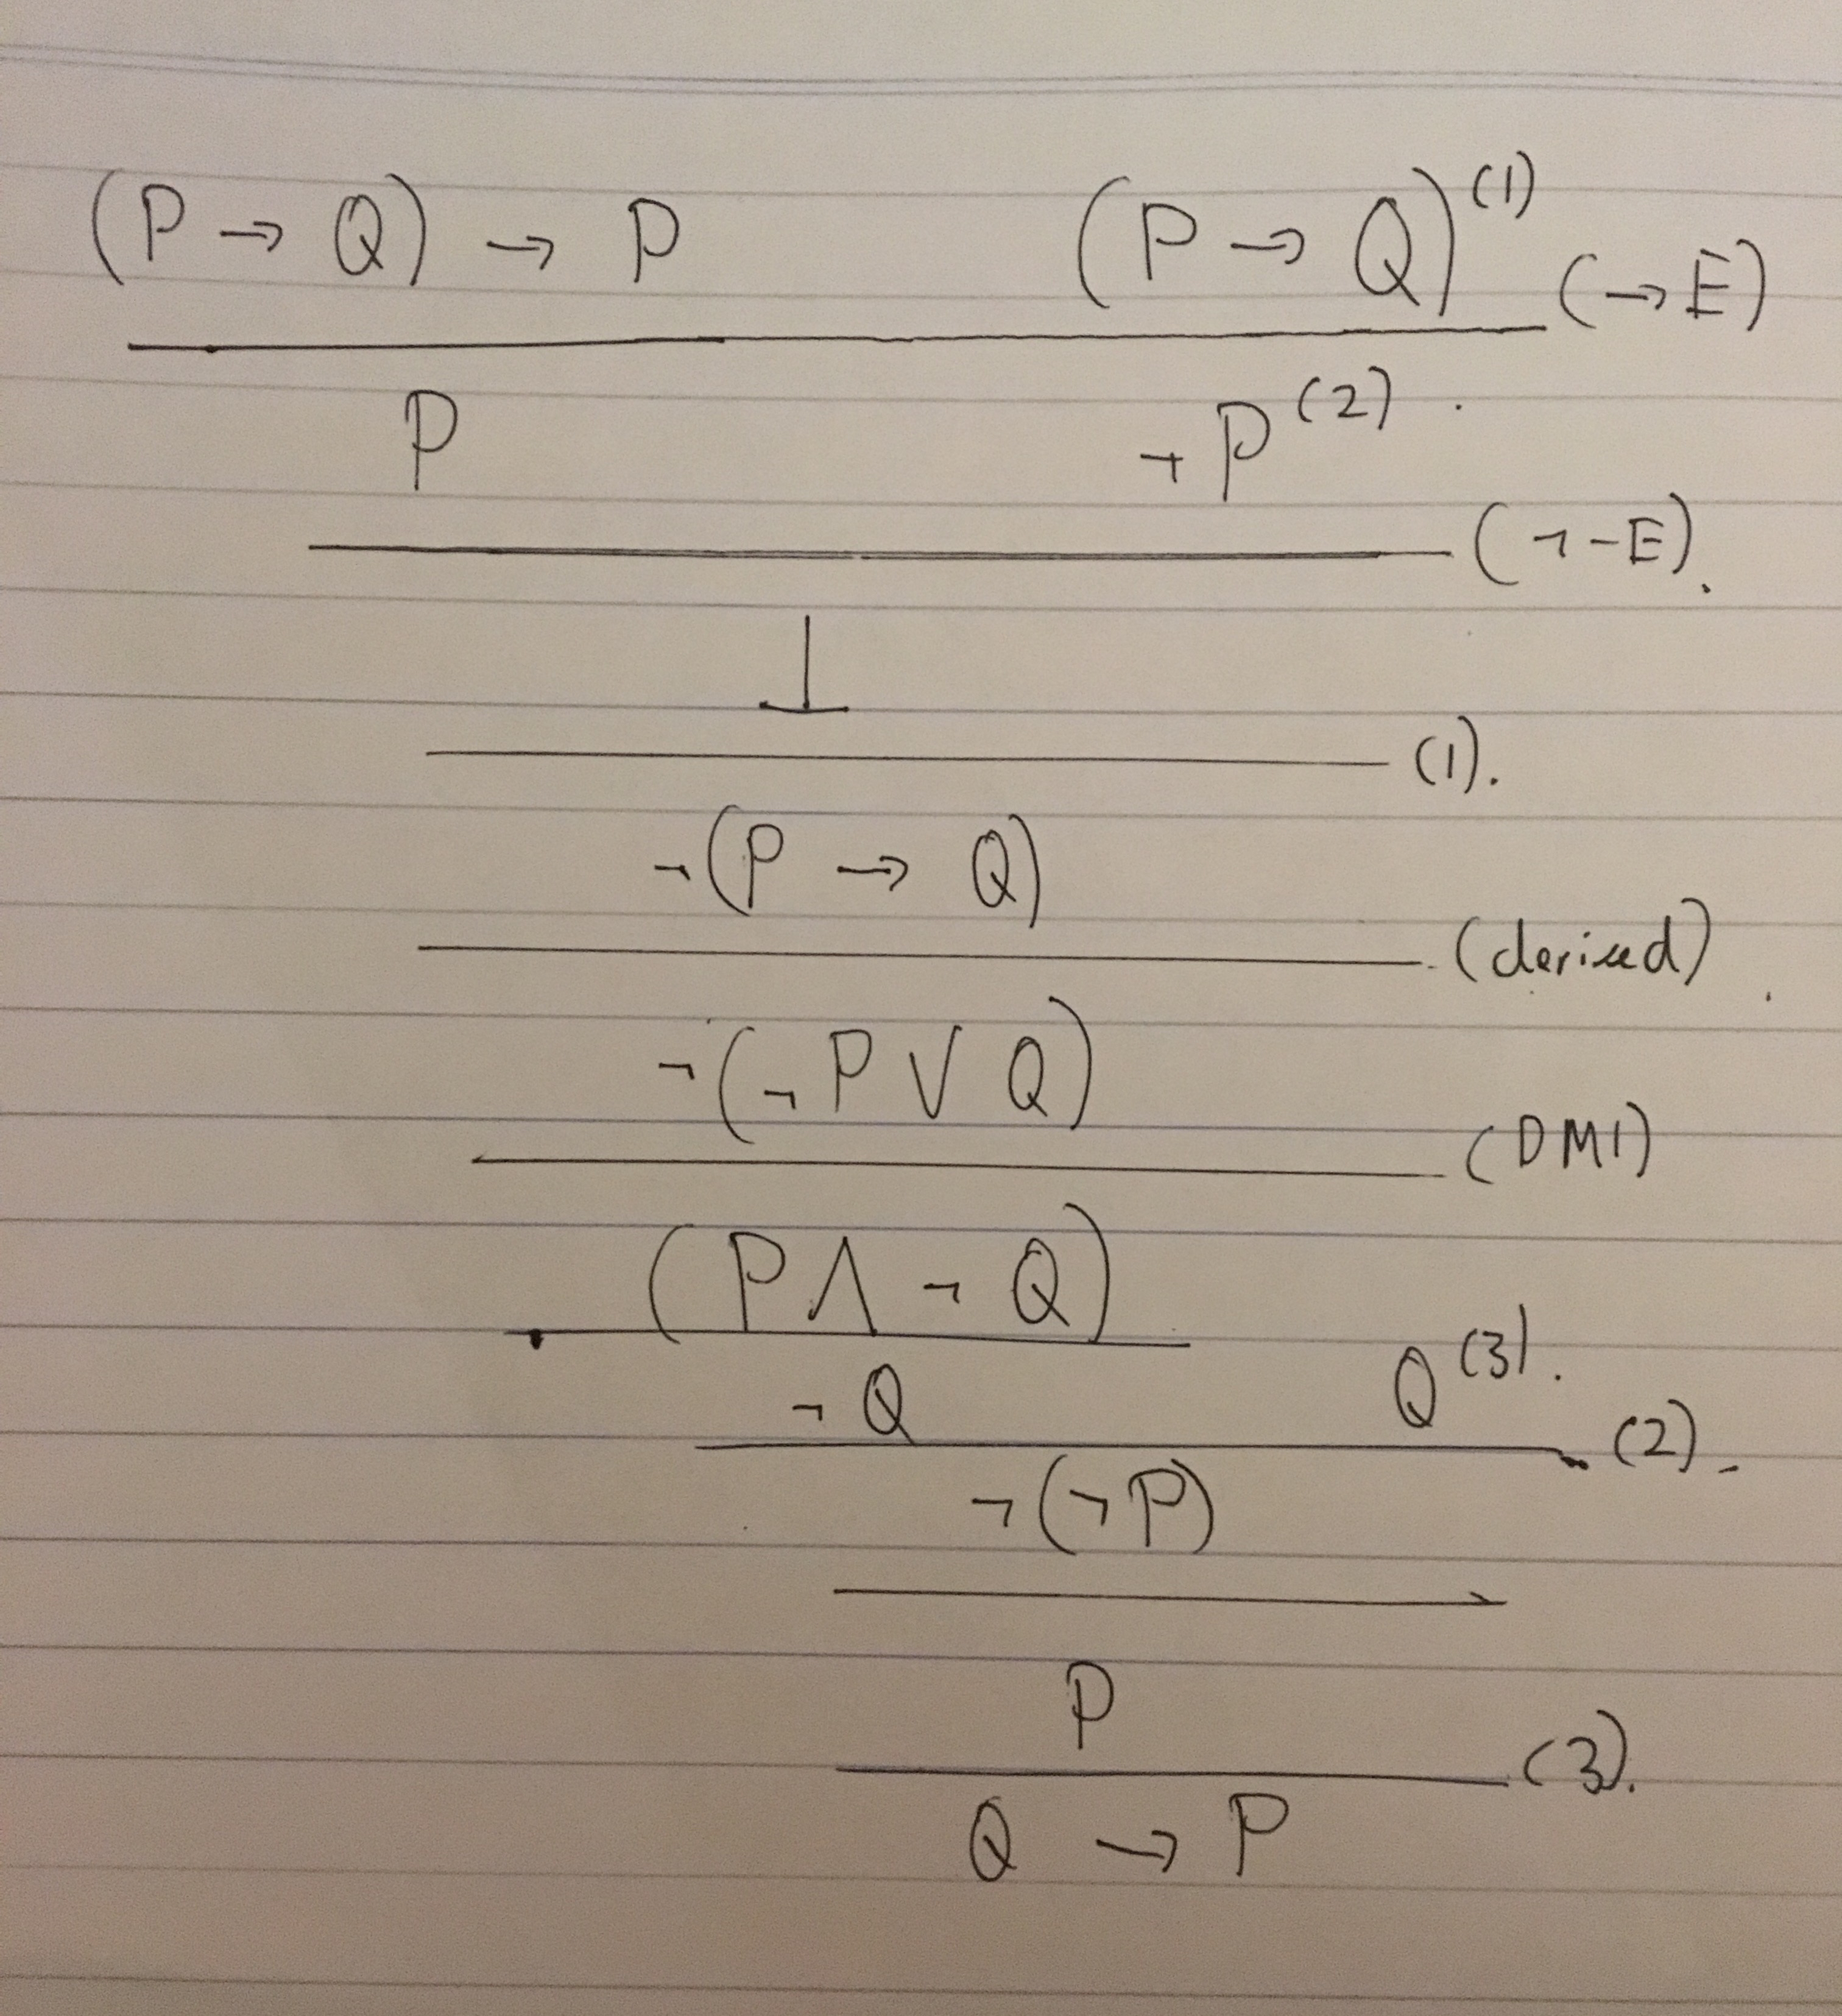
\includegraphics[width=8cm]{qimpliesp}

\subsection*{Problem 3}

Let $A$ be the range of the increasing total recursive function $f: \omega \rightarrow \omega$. We interpret ``range'' to mean the image of the function, not its co-domain.

Thus,

\[
    A = im(f) = \SET{ f(a) \mid a \in dom(f) }
\]

Recalling \textsc{Definition 190}\footnote{Page 124 of course notes} and \textsc{Defintion 191}\footnote{Page 124 of course notes}, we'll construct a function that for any $n$ will verify whether or not it is in $A$, and halts in finite time. \\

We'll reason informally about this function.\\

First, we'll assume that $im(f)$ is finite. As $f$ is increasing, it is injective. As it is injective, $dom(f)$ is finite. As $f$ is a total recursive function, it halts in finite time for all inputs in its domain. Therefore, collecting all $f(n)$ for every $n \in dom(f)$ halts in finite time. Checking membership of a finite set halts in finite time. If $a$ is in this set, $a \in A$, otherwise $a \not\in A$.\\

Secondly, we'll assume that $im(f)$ is infinite. For every $n \in dom(f)$, we compute $f(n)$ (in finite time). If $f(n) = a$, we halt, and confirm that $a \in A$. If $f(n) > a$, we halt, and confirm that $a \not\in A$. As $f$ is increasing, we can assume that some successive $n$ will never produce something that is equal to $a$ - e.g. we are allowed to halt when $f(n) > a$. As $a \in A$ describes some finite point in the ordered $\omega$, checking that $a \in A$ will halt in finite time.


\subsection*{Problem 4}

Given:

\begin{itemize}
    \item for $x \in M$, $x \text{ is regular} \Leftrightarrow x \in R^{\mathcal{M}}$
    \item for $x \in N$, $x \text{ is perfect} \Leftrightarrow x \in P^{\mathcal{N}}$
    \item Every derivation in $M$ is regular
    \item Every derivation in $N$ is perfect
\end{itemize}

We'll assume for both $\mathcal{M}$ and $\mathcal{N}$, that for each constant symbol $a$, $a^{\mathcal{M}} = a$ and $a^{\mathcal{N}} = a$

We can thus conclude that $M = R^\mathcal{M}$ and $N = P^\mathcal{N}$.

% TODO
% Given that as $\mathcal{N} \subseteq \mathcal{M}$, then $N \subseteq M$.

We can say that $\mathcal{M} \models \forall x Rx$ and $\mathcal{N} \models \forall x Px$.

\begin{enumerate}

    \item $\mathcal{N}$ has a non-empty quantifiable domain, $N$. If $\mathcal{N} \models \forall x Px$, then $\mathcal{N} \models \exists x Px$. Therefore, $\mathcal{N} \models \exists x Px$.

    \item Fix $\mathcal{M^{+}}$ such that there is some $m \in $$\LANGUAGE(C)$, such that $m^\mathcal{M^{+}} = m$, where $m \not \in P^\mathcal{M^{+}}$. $\mathcal{M^{+}}$ is a valid substitute for $\MODEL$, as it can be constructed using the rules specified prior.

        Thus, $\MODEL \not \models \forall x P x$.

    \item Note that $\forall x Rx$ is a $\Pi_1$ sentence (a $\forall$-sentence). By \textsc{Theorem 139(2)}\footnote{Page 85 of course notes}, if $\varphi$ is $\Pi_1$, and $\SUBMODEL \subseteq \MODEL$, and $\mathcal{M} \models \varphi$, then $\mathcal{N} \models \varphi$. As specified prior $\mathcal{M} \models \forall x Rx$. Therefore $\mathcal{N} \models \forall x Rx$.

    \item $\mathcal{N}$ has a non-empty quantifiable domain, $N$. If $\SUBMODEL \models \forall x Px$, then $\mathcal{N} \models \exists x Px$. For $N \subseteq M$ to be true, if $m \in P^{\SUBMODEL}$, then $m \in P^{\MODEL}$. Therefore $m \in P^{\MODEL}$. Therefore $\MODEL \models \exists x Px$. 

\end{enumerate}

\section*{Part B}

\subsection*{Problem 5}

\begin{enumerate}
    \item 

Let $\MODEL$ be a model with domain $M = \SET{}$. 


    $\not\exists x(x = x)$ is a consequence.

    Furthermore, we run into some strangeness when we find that $\forall x (x \neq x)$ is a consequence.

    $\forall x \varphi(x) \Rrightarrow \exists x \varphi(x)$ no longer holds either.

    In other words, free logic admits existentially quantified formulas always being false in the empty domain, and universally quantified formulas always being true.
    
    Furthermore, the notion that $\neg \exists x \varphi(x) \Rrightarrow \forall x \neg \varphi (x)$ ceases to be meaningful.


    \item \subsubsection*{Rules}

    We're also going to consider $\exists$ in the set logical vocabulary, because, why not?

    \begin{forest}
        [, phantom, s sep = 1cm
            [$\varphi \wedge \psi (\wedge)$
                [$\varphi ~ \psi$]
            ]
            [$\neg(\varphi \wedge \psi) (\neg \wedge)$
                [$\varphi$]
                [$\psi$]
            ]
            [$\neg\neg \varphi (\neg \neg)$
                [$\varphi$]
            ]
            [$\forall x \varphi(x) (\forall)$
                [$\neg E!a$]
                [$\varphi(a)$
                    [where $a$ is any name]
                ]
            ]
            [$\neg\forall x \varphi(x) (\neg \forall)$
                [$\exists x (\neg \varphi)(x) $]
            ]
        ]
    \end{forest}

    \begin{forest}
        [, phantom, s sep = 1cm
            [$\exists x \varphi(x) (\exists)$
                [$E!a ~ \varphi(a)$
                    [where $a$ is new]
                ]
            ]
            [$\neg\exists x \varphi(x) (\neg \exists)$
                [$\forall x (\neg \varphi)(x) $]
           ]
        ]
    \end{forest}

    where $E!c$ expands to $\exists x (x = c)$\footnote{I had to do this because the forest package wouldn't typeset leaves over a certain number of characters}.

    By new we mean that the name $a$ has not occured anywhere on the branches above.

    \item

Our goal is to show that if $\models_{f} \varphi$, then $\vdash_{Tab} \varphi$. In other words, if every model $\MODEL$ (of the language $\varphi$) is such that if $\MODEL \models \varphi$ then the tableau commencing with $\neg \varphi$ is closed.


% $\forall \gamma \in \Gamma$, $\MODEL \models \gamma$, then $\MODEL \models \varphi$, then there is a proof of $\varphi$ using assumptions among $\Gamma$.

By contraposition, if $\not\vdash_{Tab} \varphi$ then $ \not\models_{f} \varphi$.

In other words, if the tableau commencing with $\neg \varphi$ does not close, then there is some $\MODEL$ such that $M \models \neg \varphi$.

% We should show that should there be no proof of $\varphi$ from assumptions in $\Gamma$, then we can construct a set of sentences that describe a model in which $\Gamma \cup \SET{\neg \varphi}$ is true.

Rather than choosing some open branch $\mathcal{B}$ of a tableau commencing with $\neg \varphi$, and defining a $\MODEL^{\mathcal{B}}$, and reasoning with +-complexity, we'll use a $\Delta$ that is maximally consistent\footnote{for an arbitrary $\varphi$ either $\varphi \in \Delta$ or $\neg \varphi \in \Delta$} and existentially witnessed\footnote{if $\exists x \varphi(x) \in \Delta$, then for some constant symbol $a$, $\varphi(a) \in \Delta$} set of of sentences. 

Let $\MODEL^{\Delta}$ be such that:

\begin{itemize}
    \item $M^{\Delta}$ is the set of constant symbols $a$ occurring in the stentences in $\Delta$.
    \item for each constant symbol $a$, let $a^{\MODEL} = a$
    \item for each $n$-ary relation symbol $R$ of $\LANGUAGE(C)$ let $R^{\MODEL}$ be the set of $n$-tuples $\TUPLE{a_1, ..., a_n}$ such that $Ra_1,...,a_n$ is in $\Delta$.
\end{itemize}

Reiterating

\begin{claim}
    Suppose $\Delta$ is maximal consistent. Then $\varphi \in \Delta \Leftrightarrow \MODEL^{\Delta} \models \varphi$
\end{claim}

but eliding \textsc{Proof 120}\footnote{Page 77 of course notes}.

We will show $\varphi \in \Delta \Rightarrow \MODEL^{\Delta} \models \varphi$

We proceed by induction on the complexity of the forumula.

\subsubsection*{Base}

Suppose $\psi := \chi$. Then

    \begin{align*}
        \chi \in \Delta & \Leftrightarrow \MODEL^{\Delta} \models \chi
    \end{align*}

    This flows trivially from \textsc{Claim 120}.

\subsubsection*{Induction Step}

\begin{itemize}

    \item Suppose $\psi := \chi \wedge \delta \in \Delta$. 
    
    We claim that $\chi \wedge \delta \in \Delta$ iff both $\chi \in \Delta$ and $\delta \in \Delta$. 

    If $\chi \wedge \delta \in \Delta$, then by Claim 120 and tableau rule $(\wedge)$, we have both $\chi$ and $\delta$ in $\Delta$.

    \begin{align*}
        \chi \wedge \delta \in \Delta & \Rightarrow  \chi \in \Delta\ \text{and} \ \delta \in \Delta\\
        & \Leftrightarrow \MODEL^{\Delta} \models \chi\ \text{and} \ \MODEL^{\Delta} \models \delta\\
        & \Leftrightarrow \MODEL^{\Delta} \models \chi \wedge \delta
    \end{align*}

    The first $\Rightarrow$ is via our claim; the second $\Leftrightarrow$ is by induction hypothesis; and the last $\Leftrightarrow$ is from the $\models$ definition.

    \item Suppose $\psi := \neg \chi$.

    If $\chi \in \delta$, then by \textsc{Claim 120} and tableau rule $(\neg)$, $\chi \not\in \Delta$.

    \begin{align*}
        \neg \chi \in \Delta & \Leftrightarrow  \chi \not\in \Delta\\
        & \Leftrightarrow \MODEL^{\Delta} \not\models \chi\\
        & \Leftrightarrow \MODEL^{\Delta} \models \neg\chi
    \end{align*}


    The first $\Leftrightarrow$ is via the completeness of $\Delta$; the second $\Leftrightarrow$ is by the induction hypothesis; and the last is via the $\models$ definition.

    \item Suppose $\psi := \forall x \chi (x)$.

        We claim $\forall x \chi (x) \in \Delta$ for every constant symbol $a \in \LANGUAGE (C)$ such that $\chi(a) \in \Delta$.

        Suppose $\forall x \chi (x) \in \Delta$. 

        Suppose $\LANGUAGE(C) \neq \SET{}$, which given our definiton of $\MODEL^{\Delta}$, occurs when $M^{\Delta} \neq \SET{}$. 

        Then by claim \textsc{Claim 120} and tableau rule $(\forall)$ , for all $a \in \LANGUAGE(C)$, $\chi(a) \in \Delta$.

        Suppose $\LANGUAGE(C) = \SET{}$. We assert that there must be something in $\Delta$ that says there is no $a \in \LANGUAGE(C)$.
        
        Then by \textsc{Claim 120} and tableau rule $(\forall)$, there is some $\varphi$ of the form $\neg \exists y(y = a)$ such that $\varphi \in \Delta$.

        On the other hand, if for some some $a \in \LANGUAGE(C)$, $\chi (a) \in \Delta$, then by \textsc{Claim 120} and $(\forall)$, $\forall x \chi (x) \in \Delta$. 

        Then we have

    \begin{align*}
        \forall x \chi (x)\in \Delta & \Rightarrow \text{for all } a \in M^{\Delta} \text{, } \chi(a) \in \Delta \text{ or } \neg \exists y(y = a) \in \Delta\\
        & \Leftrightarrow \text{for all } a \in M^{\Delta} \text{, } \MODEL^{\Delta} \models \chi(a) \in \Delta \text{ or } \MODEL^{\Delta} \models \neg \exists y(y = a)\\
        & \Leftrightarrow \MODEL^{\Delta} \models \forall x \chi (x)
    \end{align*}

    The first $\Rightarrow$ is via our claim; the second $\Leftrightarrow$ is by induction hypothesis; and the final $\Leftrightarrow$ is was via the $\models$ definition.

    \item Suppose $\psi := \exists x \chi (x)$. 
    
        Then we claim $\exists x \chi (x) \in \Delta$ iff there is some constant symbol $a \in \LANGUAGE (C)$ such that $\chi(a) \in \Delta$.

        Suppose $\exists x \chi (x) \in \Delta$. 

        By the construction of $\Delta$\footnote{it is existentially witnessed}, \textsc{Claim 120} and tableau rule $(\exists)$, there is some $a \in \LANGUAGE(C)$ such that $\chi(a) \in \Delta$. 
        
        Furthermore we may also say that there exists some $\varphi$ of the form $\exists y(y = a)$, such that $\varphi \in \Delta$. We would not be able to say this if $\Delta$ were not existentially witnessed.

        Then we have

    \begin{align*}
        \exists x \chi (x)\in \Delta & \Leftrightarrow \text{there is some } a \in M^{\Delta} \text{ such that } \chi(a) \in \Delta \text{ and } \exists y(y = a) \in \Delta\\
        & \Leftrightarrow \text{there is some } a \in M^{\Delta} \text{ such that } \MODEL^{\Delta} \models \chi (a) \text{ and } \MODEL^{\Delta} \models \exists y(y = a)\\
        & \Leftrightarrow \MODEL^{\Delta} \models \exists x \chi (x)
    \end{align*}

    The first $\Rightarrow$ is via our claim; the second $\Leftrightarrow$ is by induction hypothesis; and the final $\Leftrightarrow$ is was via the $\models$ definition.

    The other cases are left as exercises for the marker.



\end{itemize}

\end{enumerate}




\end{document}